\documentclass[12pt]{article}
\usepackage[utf8]{inputenc}
\usepackage{amsmath}
\usepackage{amssymb}
\usepackage{graphicx}
\graphicspath{{simulations/}{./}}
\usepackage{hyperref}
\usepackage{setspace}
\usepackage[round]{natbib}
\usepackage{array}
\usepackage{tikz}
\usetikzlibrary{positioning,arrows.meta,calc,decorations.pathreplacing}
% Float placement for the review manuscript.
\renewcommand{\topfraction}{0.9}
\renewcommand{\bottomfraction}{0.8}
\renewcommand{\textfraction}{0.07}
\renewcommand{\floatpagefraction}{0.7}
\setcounter{topnumber}{2}
\setcounter{totalnumber}{3}
\setlength{\emergencystretch}{1em}
\let\oldcite\cite
\renewcommand{\cite}[1]{\citep{#1}}
\doublespacing

\title{Coupling-gated cortical coherence:\\
 a conditional framework for unity and self-representation}
\author{Sebastian Bobadilla-Suarez\\
Independent Researcher\\
\texttt{sebastian.bobadilla.s@gmail.com}\\
ORCID: \href{https://orcid.org/0000-0002-5951-0772}{0000-0002-5951-0772}}
\date{6 September 2026}
\usepackage{lineno}
% The arXiv build strips lineno; the figures call \nolinenumbers, so keep it defined.
\providecommand{\nolinenumbers}{}

\usepackage{xfp}  % \fpeval for inline Fermi-parameter arithmetic

%% Auto-generated by simulations/fermi_estimate_check.py --write-tex
%% Do not edit manually. Edit the Python script instead and regenerate.
%% Frequency-band field values from Anastassiou & Koch 2011, 2015.

% --- Global parameters ---

\newcommand{\fermiLam}{0.2}           % LFP decay length (mm)
\newcommand{\fermiLamMin}{0.1}           % measured lower bound
\newcommand{\fermiLamMax}{0.3}           % measured upper bound
\newcommand{\fermiRho}{5e+04}           % neuron density (mm$^{-3}$)
\newcommand{\fermiShift}{0.4}           % ephaptic shift per mV/mm (ms)
\newcommand{\fermiGamma}{1.5}           % Lorentzian half-width of frequency spread (rad/s)
\newcommand{\fermiThreshold}{2.0}           % $K_c/\gamma$, noiseless Lorentzian

% --- Measured field range (mV/mm) across all EEG bands ---
\newcommand{\fermiFieldMin}{1}           % 
\newcommand{\fermiFieldMax}{5}           % 

% --- Band-specific field amplitudes (mV/mm) and frequencies (Hz) ---
\newcommand{\fermiEgamma}{0.5}
\newcommand{\fermiFgamma}{40}
\newcommand{\fermiEbeta}{1.0}
\newcommand{\fermiFbeta}{20}
\newcommand{\fermiEalpha}{1.5}
\newcommand{\fermiFalpha}{10}
\newcommand{\fermiEtheta}{3.0}
\newcommand{\fermiFtheta}{6}
\newcommand{\fermiEdelta}{2.0}
\newcommand{\fermiFdelta}{2}

% --- Conservative bound parameters (low end of every range) ---
\newcommand{\fermiConsE}{1.0}           % conservative field (mV/mm)
\newcommand{\fermiConsShift}{0.3}           % conservative shift per mV/mm (ms)
\newcommand{\fermiConsLam}{0.15}           % conservative decay length (mm)
\newcommand{\fermiConsGamma}{2.0}           % conservative Lorentzian width (rad/s)

%% --- Parameterized kernel functions ---
%% \fermiK{E}{f} = coupling constant K, e.g. \fermiK{\fermiEtheta}{\fermiFgamma}
%% \fermiKGamma{E}{f} = ratio K/gamma, read against K_c/gamma = 2 (noiseless Lorentzian)
%% \fermiKGammalam{E}{f}{lam} = K/gamma with explicit lam (for range statement)
%% Nothing here divides by a phase-diffusion D: the identical-frequency noisy
%% threshold K_c = 2D is a different statement and takes a different input.

\newcommand{\fermiN}{\fpeval{round(4/3*pi*\fermiLam^3*5e+04,0)}}
\newcommand{\fermiK}[2]{\fpeval{round(4/3*pi*\fermiLam^3*5e+04 * (#1*0.4/1000) * #2, 0)}}
\newcommand{\fermiKGamma}[2]{\fpeval{round(4/3*pi*\fermiLam^3*5e+04 * (#1*0.4/1000) * #2 / \fermiGamma, 1)}}
\newcommand{\fermiKGammalam}[3]{\fpeval{round(4/3*pi*#3^3*5e+04 * (#1*0.4/1000) * #2 / \fermiGamma, 1)}}

% --- Pre-computed values used directly in prose ---
\newcommand{\fermiPhAdv}{\fpeval{round(3.0*0.4/1000*6,3)}}
\newcommand{\fermiKGammaCons}{\fpeval{round(4/3*pi*\fermiConsLam^3*5e+04 * (1.0*0.4/1000) * 40 / \fermiConsGamma, 1)}}

%% Auto-generated by simulations/simulation_tex.py
%% Do not edit manually. Run: uv run --directory simulations python simulation_tex.py

% S1: dynamic ramp
\newcommand{\rampFastEscaped}{5}
\newcommand{\rampReplicas}{32}
\newcommand{\rampDelaySlowOne}{0.1947}
\newcommand{\rampDelaySlowTwo}{0.0684}
\newcommand{\rampDelaySlowThree}{0.0253}
\newcommand{\rampDelayExponent}{0.443}
\newcommand{\rampNDelayOne}{0.0619}
\newcommand{\rampNDelayTwo}{0.1947}
\newcommand{\rampNDelayThree}{0.2341}
\newcommand{\rampNScaledDelayOne}{0.0248}
\newcommand{\rampNScaledDelayTwo}{0.0706}
\newcommand{\rampNScaledDelayThree}{0.0781}
\newcommand{\rampNPrecriticalMaxOne}{0.436}
\newcommand{\rampNPrecriticalMaxTwo}{0.223}
\newcommand{\rampNPrecriticalMaxThree}{0.106}
\newcommand{\rampOnsetPinnedOne}{true}
\newcommand{\rampOnsetPinnedTwo}{true}
\newcommand{\rampOnsetPinnedThree}{true}
\newcommand{\rampOnsetPinnedFour}{true}
\newcommand{\rampOnsetOne}{0.964}
\newcommand{\rampOnsetTwo}{0.898}
\newcommand{\rampOnsetThree}{0.471}
\newcommand{\rampOnsetFour}{0.417}
\newcommand{\rampOnsetReferenceOne}{0.443}
\newcommand{\rampOnsetReferenceTwo}{0.443}
\newcommand{\rampOnsetReferenceThree}{0.443}
\newcommand{\rampOnsetReferenceFour}{0.448}
\newcommand{\rampOnsetOrderMinOne}{0.100}
\newcommand{\rampOnsetOrderMinTwo}{0.101}
\newcommand{\rampOnsetOrderMinThree}{0.150}
\newcommand{\rampOnsetOrderMinFour}{0.133}
\newcommand{\rampOnsetOrderMaxOne}{0.151}
\newcommand{\rampOnsetOrderMaxTwo}{0.389}
\newcommand{\rampOnsetOrderMaxThree}{0.382}
\newcommand{\rampOnsetOrderMaxFour}{0.399}
\newcommand{\rampOnsetExcessMinOne}{0.32}
\newcommand{\rampOnsetExcessMinTwo}{0.04}
\newcommand{\rampOnsetExcessMinThree}{0.01}
\newcommand{\rampOnsetExcessMinFour}{0.00}
\newcommand{\rampOnsetExcessMaxOne}{0.50}
\newcommand{\rampOnsetExcessMaxTwo}{0.31}
\newcommand{\rampOnsetExcessMaxThree}{0.19}
\newcommand{\rampOnsetExcessMaxFour}{0.20}
\newcommand{\rampOnsetSamplesOne}{19}
\newcommand{\rampOnsetSamplesTwo}{28}
\newcommand{\rampOnsetSamplesThree}{19}
\newcommand{\rampOnsetSamplesFour}{200}
\newcommand{\rampCollapseOne}{0.00245}
\newcommand{\rampCollapseTwo}{0.00599}
\newcommand{\rampCollapseThree}{0.00689}
\newcommand{\rampCollapseFour}{0.00705}
\newcommand{\rampCollapseThreshold}{0.01410}

% S2: spatial kernel
\newcommand{\spatialCriticalDecay}{0.0140}
\newcommand{\spatialCriticalDecayCells}{0.90}
\newcommand{\spatialPlateauMax}{8.0}
\newcommand{\spatialOrderOne}{0.9424}
\newcommand{\spatialOrderTwo}{0.9427}
\newcommand{\spatialOrderThree}{0.9427}
\newcommand{\spatialDefectMaximum}{2.4\times10^{-6}}

% S3: dynamical selection
\newcommand{\selectionSubOrder}{0.06266}
\newcommand{\selectionCriticalOrder}{0.16049}
\newcommand{\selectionSuperOrder}{0.67735}
\newcommand{\selectionTheoryOrder}{0.68270}
\newcommand{\selectionStaticResidual}{-0.00535}
\newcommand{\selectionSuperOrderDtHalf}{0.68021}
\newcommand{\selectionStaticResidualDtHalf}{-0.00250}
\newcommand{\selectionRateSlope}{0.41505}
\newcommand{\selectionRateIntercept}{-0.78619}
\newcommand{\selectionWindowLowerBase}{0.06325}
\newcommand{\selectionWindowUpperBase}{0.20669}

% S4: propagation of chaos
\newcommand{\chaosNMin}{10}
\newcommand{\chaosNMax}{1000}
\newcommand{\chaosSubOrderLowN}{0.3726}
\newcommand{\chaosSubOrderHighN}{0.0402}
\newcommand{\chaosSubCorrelationLowN}{0.0458}
\newcommand{\chaosSubCorrelationHighN}{0.0010}
\newcommand{\chaosSubDistanceLowN}{0.0468}
\newcommand{\chaosSubDistanceHighN}{0.0419}
\newcommand{\chaosSubDensityLowN}{0.2640}
\newcommand{\chaosSubDensityHighN}{0.1286}
\newcommand{\chaosSuperOrder}{0.7208}
\newcommand{\chaosSuperCorrelationMin}{0.459}
\newcommand{\chaosSuperCorrelationMax}{0.525}
\newcommand{\chaosSuperDistanceLowN}{0.1042}
\newcommand{\chaosSuperDistanceHighN}{0.0812}
\newcommand{\chaosMeasuredConcentration}{2.1624}
\newcommand{\chaosDensityError}{0.1291}
\newcommand{\chaosBesselResidual}{0.00191}
\newcommand{\chaosRuntimeSeconds}{1622.35}

% S5: conditional frustration rescue
\newcommand{\frustrationBaselineMin}{0.0508}
\newcommand{\frustrationBaselineMax}{0.0574}
\newcommand{\frustrationCouplingMin}{1.8994}
\newcommand{\frustrationCouplingMax}{1.9387}
\newcommand{\frustrationBracketMin}{1.857}
\newcommand{\frustrationBracketMax}{2.110}
\newcommand{\frustrationGridRatio}{1.136}
\newcommand{\frustrationFieldOneMin}{0.5668}
\newcommand{\frustrationFieldTwoMin}{0.0709}
\newcommand{\frustrationFieldThreeMin}{0.0210}
\newcommand{\frustrationFieldOneMax}{0.5785}
\newcommand{\frustrationFieldTwoMax}{0.0723}
\newcommand{\frustrationFieldThreeMax}{0.0214}

% S6: joint phase/plasticity dynamics
\newcommand{\plasticityOrderMin}{0.9167}
\newcommand{\plasticityOrderMax}{0.9222}
\newcommand{\plasticityDissipationMin}{1110.5659}
\newcommand{\plasticityDissipationMax}{1116.6277}
\newcommand{\plasticityDescentMin}{0.6773}
\newcommand{\plasticityDescentMax}{0.6914}
\newcommand{\plasticityRatioInitialMin}{0.9824}
\newcommand{\plasticityRatioInitialMax}{0.9948}
\newcommand{\plasticityRatioMin}{0.3507}
\newcommand{\plasticityRatioMax}{0.6135}
\newcommand{\plasticityPercentileMin}{0.9510}
\newcommand{\plasticityPercentileMax}{1.0000}
\newcommand{\plasticityNormGrowthMin}{12.4094}
\newcommand{\plasticityNormGrowthMax}{14.6958}
\newcommand{\plasticityReductionMin}{-58.0962}
\newcommand{\plasticityReductionMax}{-48.1760}
\newcommand{\plasticityCorrelationMin}{-0.0362}
\newcommand{\plasticityCorrelationMax}{-0.0208}
\newcommand{\plasticityRandomDescentMin}{-0.0173}
\newcommand{\plasticityRandomDescentMax}{-0.0103}
\newcommand{\plasticityRandomRatioMin}{0.9965}
\newcommand{\plasticityRandomRatioMax}{0.9997}
\newcommand{\plasticityRandomNormGrowthMin}{1.2879}
\newcommand{\plasticityRandomNormGrowthMax}{1.3056}
\newcommand{\plasticityFrozenDissipationMin}{1380.6063}
\newcommand{\plasticityFrozenDissipationMax}{1382.3448}
\newcommand{\plasticityFrozenPercentileMin}{0.6435}
\newcommand{\plasticityFrozenPercentileMax}{0.9110}
\newcommand{\plasticitySigmaFloor}{990}
\newcommand{\plasticityLearningRate}{0.2}
\newcommand{\plasticitySweepLowRate}{0.001}
\newcommand{\plasticitySweepHighRate}{0.4}
\newcommand{\plasticitySweepBestRate}{0.2}
\newcommand{\plasticitySweepLowDissipation}{1377.9075}
\newcommand{\plasticitySweepHighDissipation}{1248.2272}

% Empirical (a, r) collapse: what the observed range discriminates
\newcommand{\collapseLinearDeviation}{0.0095}
\newcommand{\collapseTanhDeviation}{0.0030}
\newcommand{\collapseProbe}{1.5}
\newcommand{\collapseProbeSeparation}{0.154}
\newcommand{\collapseTarget}{0.17}
\newcommand{\collapseTargetConcentration}{1.56}


\begin{document}
\begingroup
\singlespacing
\maketitle
\endgroup

\begin{abstract}
\singlespacing
How could coordinated cortical activity support a unified experience and a minimal self? We develop a conditional field framework separating three requirements: coherence, compatibility and self-representation. Its physical hypothesis is that endogenous extracellular fields partly couple cortical processes, with changing extracellular geometry gating recovery after awakening. A noisy mean-field phase model predicts a square-root stationary onset and a von Mises concentration--coherence relation. Finite ramps delay that onset, and increased coupling, decreased diffusion and a matched common drive can give identical stationary phase distributions. A test therefore needs calibrated phase dynamics and measurements that distinguish the interaction mechanism. Beyond coherence, an explicit counterexample shows that phase agreement permits incompatible local states; a plasticity control preserves coherence while losing alignment with specified environmental structure. Compatible spatial measures glue uniquely, and a contracting self-prediction map has a unique fixed point, each relative to supplied local data and model choices. Lean~4 checks their composition under eight connecting hypotheses and supplied structures. We motivate the identification of the glued state with conscious unity and of its accurate self-representation with a minimal self. The framework specifies what each requirement contributes and which additional measurements would make those identifications assessable.
\end{abstract}
\linenumbers

\section{Introduction}

How could activity distributed across cortex support one experience? A field account proposes that endogenous extracellular electromagnetic fields partly coordinate spatially separated neural processes \cite{mcfadden2002,mcfadden2020,pockett2012}. Ephaptic effects provide a possible interaction mechanism \cite{frohlich2010,anastassiou2015}. Yet even successful coordination leaves a question: what makes the coordinated activity a description of one experienced situation, with a perspective on that situation?

We separate three requirements. \emph{Coherence} concerns whether coupling sustains collective activity. \emph{Compatibility} concerns whether local descriptions agree where their domains overlap, so they can belong to a single global description. \emph{Self-representation} concerns whether that global state supports an accurate model of itself. These requirements organize the article. They are commitments of the construction developed here; they are not offered as requirements on every possible account of consciousness.

The distinction between timing and content is central. Imagine two local descriptions assigning different values to the same shared quantity. Making their oscillations synchronous leaves that disagreement intact. The formal construction exhibits exactly this separation: local spatial mass profiles at a common phase can disagree on an overlap. Equal restrictions, rather than equal phases, allow those profiles to glue into a unique global state. A self-prediction map then asks a further question about that state: can a local encoding reproduce the state of which it is a part?

Awakening gives the physical requirement a concrete setting. We hypothesize that changing extracellular geometry slowly increases effective coupling through a synchronization threshold. Under stationary branch tracking, a noisy phase model fixes a square-root onset of coherence. The experiment faces two distinct obstacles. Finite ramp speeds delay the response, so a fitted onset exponent depends on the drive. Moreover, successive stationary phase distributions can be identical under increasing coupling, decreasing diffusion or a suitably matched common drive. Recovery must therefore be measured in a way that identifies dynamics and distinguishes causes, rather than inferred from the shape of a coherence trace alone.

The next requirement is representational. A plasticity control shows why an adaptive coherent system need not acquire the environmental structure it is scored against: a squared-drift objective rewards equalizing drift, which in the chosen frequency-cluster model favors connections across the clusters that define the template. This result motivates an explicit compatibility condition and a measurement of that condition. It also locates the role of thermodynamics: bounds on information and dissipation constrain an implementation, while the content its variables represent requires additional structure.

The final requirement connects unity to a minimal self. We propose that a global state fixed by its own local encoding and readout is a formal correlate of a state that is what it takes itself to be. The proposal earns its interest by requiring the self-model to refer to the same state assembled from local descriptions. Its psychological interpretation depends on identifying the relevant descriptions, their domains and the encoding region. These choices receive explicit attention in Section~\ref{sec:self}.

Lean~4 checks the mathematical composition underlying this account. Its value is to keep different objects and claims distinct: a stationary density and a trajectory, a dissipation bound and a learning rule, phase agreement and agreement of local descriptions. The composition consumes eight named connecting hypotheses and two structures with further physical content; a witness assembled from distinct toy components satisfies them jointly. Section~\ref{sec:chain} explains those obligations and the supporting thermodynamic results. The empirical tests concern the physical coherence hypothesis; the interpretation of a compatible, self-representing state as a conscious episode is argued in Section~\ref{sec:commitment}. Figure~\ref{fig:chain} gives the structure of the argument.

\begin{figure}[htbp]
\centering
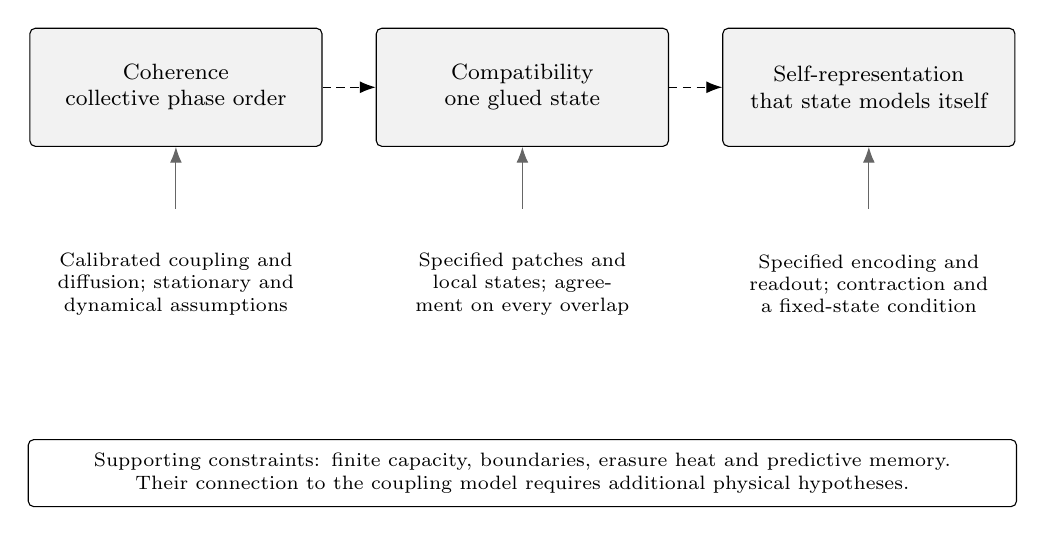
\begin{tikzpicture}[
 font=\footnotesize,
 result/.style={draw, rounded corners=2pt, align=center, text width=35mm,
                minimum height=15mm, inner sep=3pt, fill=black!5},
 input/.style={align=center, text width=35mm, minimum height=19mm,
               inner sep=3pt, font=\scriptsize},
 assumption/.style={-{Latex[length=2mm]}, densely dashed},
 supplied/.style={-{Latex[length=2mm]}, black!60}
]
\nolinenumbers
\node[result] (coherence) at (0,0) {Coherence\\collective phase order};
\node[result] (unity) at (44mm,0) {Compatibility\\one glued state};
\node[result] (self) at (88mm,0) {Self-representation\\that state models itself};
\node[input] (physical) at (0,-25mm) {Calibrated coupling and diffusion; stationary and dynamical assumptions};
\node[input] (cover) at (44mm,-25mm) {Specified patches and local states; agreement on every overlap};
\node[input] (map) at (88mm,-25mm) {Specified encoding and readout; contraction and a fixed-state condition};
\draw[supplied] (physical) -- (coherence);
\draw[supplied] (cover) -- (unity);
\draw[supplied] (map) -- (self);
\draw[assumption] (coherence) -- (unity);
\draw[assumption] (unity) -- (self);
\node[draw, rounded corners=2pt, align=center, text width=122mm,
      inner sep=5pt, font=\scriptsize] at (44mm,-49mm)
 {Supporting constraints: finite capacity, boundaries, erasure heat and predictive memory.\\
 Their connection to the coupling model requires additional physical hypotheses.};
\end{tikzpicture}
\caption{Three requirements of the proposed account. Each requires the inputs shown below it. Dashed arrows mark proposed connections: phase coherence alone supplies neither compatible local descriptions nor an accurate self-model. Thermodynamics constrains a candidate implementation through separate assumptions. This is the explanatory structure of the article; Table~\ref{tab:summary} records the eight implications consumed by the formal composition.}
\label{fig:chain}
\end{figure}

\section{Coherence: the coupling model}
\label{sec:field}

\subsection{Dynamics and the stationary threshold}

The finite stochastic model is
\begin{equation}
 d\theta_i=\left[\omega_i+\sum_j K_{ij}(t)\sin(\theta_j-\theta_i)\right]dt
 +\sqrt{2D}\,dW_i,
 \qquad
 r_N=\left|\frac1N\sum_i e^{i\theta_i}\right|.
\end{equation}
Here $D>0$ is phase diffusion, $W_i$ are independent Wiener processes, and $K_{ij}$ has inverse-time units, with angles dimensionless. The uniform mean-field convention is $K_{ij}=K/N$. Frequency heterogeneity and phase diffusion are separate parameters.

For identical frequencies in their rotating frame, the stationary ansatz is
\begin{equation}
 \rho(\theta)=\frac{e^{a\cos(\theta-\psi)}}{2\pi I_0(a)},
 \qquad a=\frac{Kr}{D},\qquad
 r=R(a):=\frac{I_1(a)}{I_0(a)},
 \label{eq:selfconsistency}
\end{equation}
where $I_n$ are modified Bessel functions and $\psi$ is the collective phase. Lean verifies normalization, the circular order parameter and self-consistency for this density. At $K\leq K_c=2D$, the only nonnegative self-consistent order parameter is zero. At $K>K_c$, exactly one positive solution coexists with zero; it emerges continuously and increases strictly with $K$. Near threshold,
\begin{equation}
 \frac{r^2}{K-K_c}\longrightarrow\frac1D,
 \qquad r\sim\sqrt{\frac{K-K_c}{D}}.
 \label{eq:onset}
\end{equation}
These results characterize the stationary branch (Fig.~\ref{fig:bifurcation}). Connecting it to finite trajectories requires a dynamical mean-field limit and dynamical selection, neither proved here. Propagation of chaos concerns the first of these steps \cite{sznitman1991}; exchange symmetry alone does not establish independence, especially when realizations have an unpinned collective phase.

\begin{figure}[htbp]
\centering
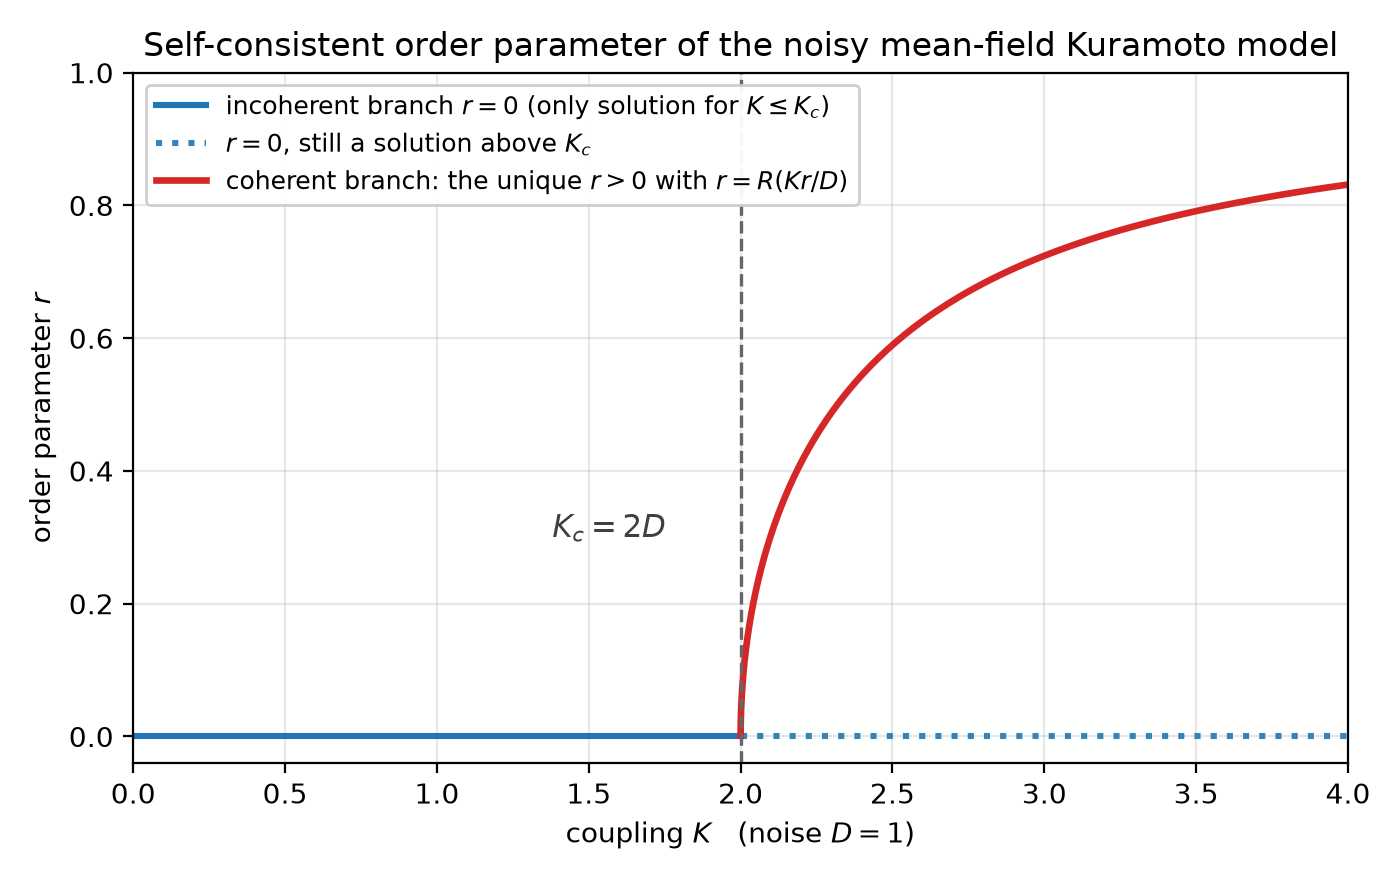
\includegraphics[width=0.80\linewidth]{bifurcation_diagram.png}
\caption{Stationary self-consistency for identical frequencies and phase diffusion $D=1$. The positive coherent branch appears continuously above $K_c=2D$ and increases with coupling. Zero remains a solution above threshold. The curve is computed from the integral expressions used in the formalization.}
\label{fig:bifurcation}
\end{figure}

A spatial version replaces the finite sum by an integral against a kernel $K(x,y)$. The substrate measure has total mass one, making the mean-field strength a kernel average. Applying the scalar threshold to a heterogeneous or signed kernel requires a justified reduction to that mean-field description.

\subsection{Physical identification and calibration}
\label{sec:scaling}

The cortical hypothesis identifies part of the effective coupling with endogenous extracellular electromagnetic interactions. Fields can modulate spike timing \cite{frohlich2010,anastassiou2015}, and field models have been proposed for coordinating distributed neural information \cite{pinotsis2022,mcfadden2020}. The quantitative question is whether that interaction supplies sufficient coupling relative to diffusion. Changes in phase organization under propofol \cite{bastos2021} motivate studying this regime, but do not measure the coupling itself.

The physical field predicate requires a jointly continuous kernel, a normalized substrate, a mean-field strength equal to the spatial average, and no single site providing more than half that strength. Regular mesh refinement establishes convergence of a scalar coupling-energy quadrature; constructing the kernel and relating it to trajectories are separate modelling tasks. The formal witnesses supply toy instances of the predicate.

Calibration is essential because a spike-time shift is not a coupling rate. An estimate proportional to $N\Delta t f$, using population size, timing shift and oscillation frequency, is dimensionless. A conversion of the form
\begin{equation}
 K_{\mathrm{eff}}=\gamma N s E f
 \label{eq:keff}
\end{equation}
requires a rate $\gamma$, where $s$ is the timing shift per unit field and $E$ the field amplitude. This rate specifies how induced timing shifts persist and accumulate into phase drift. Supplemental Material explains why the other factors cannot determine it. The biological threshold test requires independent estimates of the interaction kernel, its aggregation, and phase diffusion in the same cortical regime.

\section{Testing coherence through recovery after awakening}
\label{sec:prediction}

The proposed control variable is extracellular geometry. Sleep-associated changes in extracellular space and clearance \cite{xie2013} motivate a coupling parameter that evolves more slowly than phase dynamics. The extracellular volume fraction is approximately $\alpha=0.2$ at diffusion tortuosity $\lambda\approx1.6$ \cite{sykova2008}; the cited sleep study reports a rise in $\alpha$ from roughly $0.14$ to $0.23$ \cite{xie2013}. Below $10$\,kHz cortical tissue conducts approximately resistively at $0.3$--$0.6$\,S\,m$^{-1}$ \cite{barbour2017}. In an effective-medium description at fixed transmembrane current density, a larger extracellular volume fraction raises conductivity and reduces field amplitude.

This gives the coupling-gated hypothesis a directional prediction: contraction of extracellular space on awakening raises $E$ and, with the other factors in Eq.~\eqref{eq:keff} held fixed, raises effective coupling. The proposed geometry--coupling relation and its role in human recovery both require measurement. The effective-medium argument supplies a sign under stated conditions; calibration supplies the magnitude and the mapping to the scalar model.

If $K(t)$ rises through $K_c$ and the phase distribution tracks the coherent stationary branch, Eq.~\eqref{eq:onset} gives
\begin{equation}
 r(t)\sim\sqrt{\frac{\dot K(t_0)}{D}}\,(t-t_0)^{1/2},
 \qquad t>t_0,\quad \dot K(t_0)>0.
 \label{eq:recovery}
\end{equation}
The crossing time satisfies $K(t_0)=K_c$. It is a prediction of latency only when coupling is measured independently of coherence. The subsequent shape and saturation depend on the later coupling trajectory. Critical slowing down restricts branch tracking near threshold, while finite populations have fluctuating order below it. A measurable onset therefore needs an explicit criterion above that fluctuation floor.

\subsection{What a recovery distribution can identify}
\label{sec:identifiability}

Equation~\eqref{eq:selfconsistency} gives a concentration--coherence relation with no fitted shape parameter. Testing it requires separate estimators: $r$ from circular resultant length and $a$ from density shape. Estimating $a$ by inverting $R$ from the measured $r$ makes agreement automatic. Even a valid agreement tests a statistical description shared by the von Mises family; it does not determine the coupling medium.

There is a stronger limitation. Successive equilibrated phase distributions cannot, by themselves, distinguish three different recovery mechanisms. Let $q(t)$ be a prescribed ratio crossing $2$, let $r(q)$ denote its stationary branch, and choose a fixed rate $D_0>0$. Increasing coupling with $K(t)=D_0q(t)$ and $D=D_0$ gives the same stationary density as fixed coupling $K_0$ with decreasing diffusion $D(t)=K_0/q(t)$. Both have concentration $a=q(t)r(q(t))$. Uncoupled oscillators under a common prescribed drift $-h(t)\sin(\theta-\psi)$, with $h(t)=D_0q(t)r(q(t))$ and $D=D_0$, have that same density. Their distributions coincide window by window, even though their physical causes differ. Supplemental Material supplies the construction and its numerical feasibility check.

The missing observable is the physical clock. Resolved phase increments contain rate information: in the ideal continuous-path model, quadratic variation accumulates at rate $2D$, while conditional increment means constrain drift. This can separate coupling and diffusion under the specified observation model. Distinguishing endogenous coupling from the matched common drive additionally requires a measured drive or a controlled perturbation, because their mean-field drifts can coincide. Identifying the coupling as electromagnetic then requires evidence specific to that interaction. This hierarchy determines the experiment: distribution, dynamics and physical mechanism are distinct targets.

\subsection{Finite ramps change the observable onset}
\label{sec:numerics}
\label{sec:ramp}

Finite simulations characterize how the stationary prediction can appear in a recovery measurement. Their numerical results are generated from saved summaries; the supplement gives parameters, estimators and further controls. The ramp study uses $N=2000$, $D=1$ and 32 replicas at four coupling speeds. Escape is the first of three consecutive saved samples at $r\geq0.2$ after threshold.

Faster ramps delay escape (Fig.~\ref{fig:ramp}). Only $\rampFastEscaped/\rampReplicas$ replicas escape within the fastest window. The three slower ramps have mean coupling delays $\rampDelaySlowOne$, $\rampDelaySlowTwo$ and $\rampDelaySlowThree$. Their fitted onset exponents run from $\rampOnsetTwo$ to $\rampOnsetFour$, compared with $\rampOnsetReferenceTwo$ to $\rampOnsetReferenceFour$ from the same estimator on the exact stationary branch at the same coupling grids. At the fastest speed the ensemble mean never reaches the declared fit window; the returned value $\rampOnsetOne$ is a local log-slope of a delayed trajectory.

This is delayed passage through a noisy bifurcation \cite{berglund2002}, with a direct consequence for the awakening test: the apparent exponent depends on the ramp and on the fitting window. A deviation from the square-root law constrains the adiabatic approximation only where branch tracking is independently justified. The sweep does not bracket the specified deviation-based critical ramp speed.

\begin{figure}[htbp]
\centering
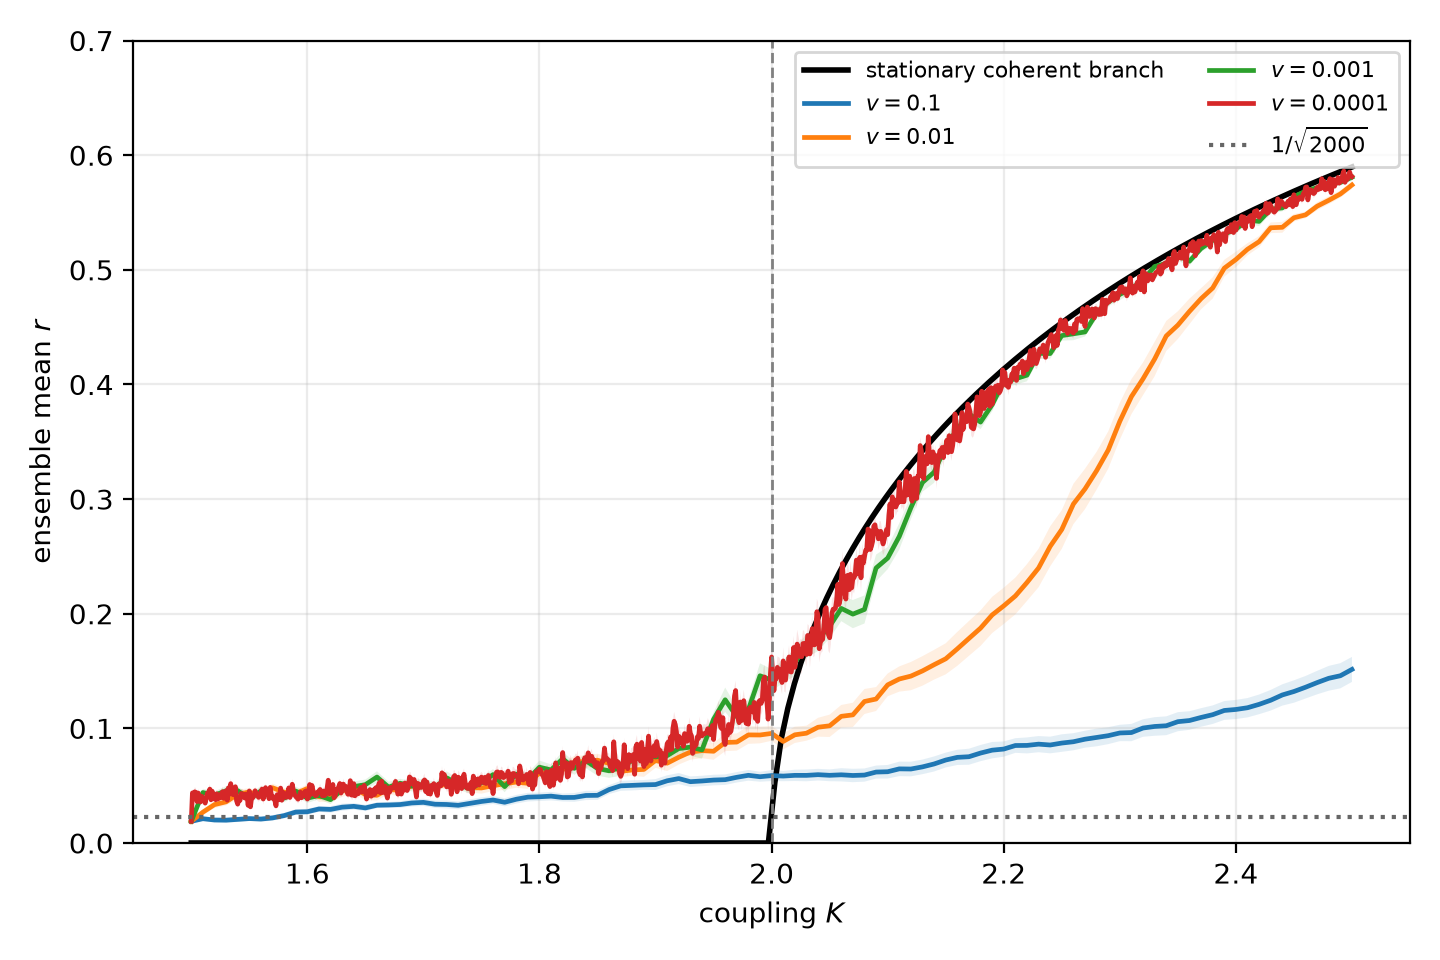
\includegraphics[width=0.90\linewidth]{figures/dynamic_ramp_bifurcation_delay.png}
\caption{Finite-rate departures from the stationary branch. Ensemble-mean order versus coupling for four ramp speeds $v$, with one-standard-error bands across replicas. The dashed vertical line is the static threshold and the dotted horizontal line the finite-size reference. Faster ramps delay escape, changing the apparent recovery onset.}
\label{fig:ramp}
\end{figure}

Additional controls test the approximations used by the physical model. Time-step refinement attributes most of the sampled discrepancy from the stationary order to integration bias. Population-size diagnostics show why a shared random collective orientation can preserve unconditional pair correlation in the coherent regime. Spatial and signed-network controls exhibit coherence at specified total coupling, with the refined signed-network crossing bracket $K_{\mathrm{eff}}/D\in[\frustrationBracketMin,\frustrationBracketMax]$ still containing $2$. These controls delimit finite regimes and numerical resolution; the supplement reports their full evidence. Calibrating the cortical coupling remains the experimental task.

\subsection{What the estimators produce on EEG}

Public propofol-sedation EEG \cite{bajwa2025} provides an exploratory exercise of the concentration and coherence estimators. The implemented analysis pools channels over 100-ms windows, estimating a spatiotemporal phase distribution. Bipolar and common-reference montages produce different residuals. The bipolar results are compatible with the Bessel relation, but the concentration range is too narrow to distinguish it from its linear approximation at the observed scatter.

An informative recording needs a broader concentration range, estimator calibration that accounts for dependence, and an observation model for source mixing, referencing and temporal pooling. The sleep-recovery hypothesis remains untested by these sedation recordings.

\subsection{A protocol for the awakening experiment}
\label{sec:protocol}

The analysis defines six requirements for the physical test.
\begin{enumerate}
\item \textbf{Coupling and diffusion in the same units.} Estimate $K$ and $D$ from resolved phase dynamics in the same cortical regime, separating diffusion, frequency heterogeneity and observation noise. A measured drive or controlled perturbation is additionally needed to distinguish endogenous coupling from the matched common-drive alternative.
\item \textbf{Geometry calibrated to coupling.} Establish the relation between an extracellular-geometry observable and effective coupling, with uncertainty. A diffusion-MRI or astrocytic proxy for volume fraction requires its own validation; the conductivity argument supplies only the expected sign.
\item \textbf{Adequate phase measurements.} For the proposed spatial estimator, use at least 100 sites per estimate, $r$ from resultant length, and $a$ from unweighted regression of log density on the cosine of centered phase. This numerical minimum needs null calibration at the actual sample count, concentration range and dependence. Temporal pooling changes the estimand.
\item \textbf{An independent recovery endpoint.} Measure behavioral recovery separately from the phase trace.
\item \textbf{A predeclared onset criterion.} Fix a coherence threshold above the finite-size floor and account for finite ramp speed before interpreting an onset exponent.
\item \textbf{Matched model comparison.} Compare coupling-gated recovery with diffusion change, common drive and alternative slow-recovery models under the same observation and filtering assumptions. Stationary distributions alone cannot resolve the equivalence in Section~\ref{sec:identifiability}.
\end{enumerate}

Failure of the concentration--coherence relation over an informative range would constrain the phase-density model. Failure of the calibrated geometry--coupling association would constrain the proposed physical gate. A competing dynamical explanation that better predicts independently measured recovery would count against its role in awakening. These tests address the first requirement of the framework. Even a favorable outcome leaves the question of what the coordinated activity represents.

\section{Compatibility: from coordinated activity to a global description}
\label{sec:unity}

\subsection{Why common timing is insufficient}

Consider overlapping patches $U$ and $V$, each carrying a local description. Compatibility requires that restricting either description to $U\cap V$ gives the same object. Agreement concerns the shared domain; descriptions on distinct parts can remain different. For the finite spatial measures used here, equal overlap restrictions give a unique measure on the covered domain. This is the gluing property formalized by a sheaf.

The formal counterexample makes the additional requirement visible. Every patch has the same oscillator phase, yet two local mass profiles assign different densities to a shared site. They cannot be restrictions of a single global measure. Phase order therefore cannot establish compatibility. Continuity of a physical field does not repair disagreement in the descriptions associated with it.

For a theory of experience, the attraction of gluing is that local contents contribute to one description without each region having to carry that entire description. Its mathematical realization here is deliberately specific: the objects are spatial measures. A decoder assigning probability laws to perceptual contents needs a further extension model, because matching overlap marginals need not determine a unique global joint distribution \cite{abramsky2011}. The passage from spatial profiles to content-bearing neural descriptions is consequently a substantive modelling commitment.

\subsection{Coherent adaptation can lose environmental alignment}
\label{sec:plasticity}

An adaptive coupling rule might appear to supply that missing representational structure. The squared-drift control shows why the objective matters. Symmetric coupling conserves mean drift: pairwise sine terms cancel when summed over nodes. Minimizing the sum of squared drifts at that fixed mean therefore rewards equalizing drift across nodes. In the chosen frequency-cluster model, this favors coupling between unlike-frequency clusters, whereas the diagnostic template rewards coupling within like-frequency clusters. The objective and the scored structure pull in different directions.

For fixed phases, the continuum objective is
\begin{equation}
 \sigma(K)=\frac1D\int\left[\omega(x)+\int K(x,y)\sin(\theta_y-\theta_x)\,d\mu(y)\right]^2d\mu(x).
\end{equation}
The formalization constructs the bounded drift operator $A$ and its adjoint, obtains $\nabla\sigma=(2/D)A^*(AK+\omega)$, and proves descent for the specified gradient flow. This is a squared-drift functional; identifying thermodynamic entropy production would require probability-current information.

The finite control co-evolves noisy phases and symmetric, nonnegative couplings at fixed total resource. Across three seeds it compares gradient updates, random updates scaled to each arm's own gradient norm, randomly relabelled gradient updates, and a frozen kernel. The frequency-cluster template is a diagnostic covariance of shared latent signals, not a training input. Figure~\ref{fig:resonance} shows the decisive dissociation: second-half order remains between $\plasticityOrderMin$ and $\plasticityOrderMax$, while the within-cluster to between-cluster coupling ratio falls from $\plasticityRatioInitialMin$--$\plasticityRatioInitialMax$ to $\plasticityRatioMin$--$\plasticityRatioMax$. The relabelled arm reaches overlapping deformation and coherence ranges but a ratio of $\plasticityPermutedRatioMin$--$\plasticityPermutedRatioMax$, above the gradient arm's range. Supplementary controls compare partitions blind to frequency and distinguish alignment from growth of the kernel norm.

The objective reduction is transient. Immediately after updates, the gradient arm removes a fraction $\plasticityDescentMin$--$\plasticityDescentMax$ of the headroom above the conserved-drive floor. Averaging over complete update intervals removes that apparent sustained gain. A prespecified grid of $\plasticityStudyCaseCount$ rate--cadence combinations contains no case meeting the declared $5\%$ sustained-reduction criterion while retaining coherence and losing alignment. The evidence therefore concerns coherent adaptation away from a specified structure, not sustained minimization of a thermodynamic cost.

This control is not a test of overlap compatibility itself: kernel alignment and agreement of local descriptions are different observables. Its role is to block a proposed shortcut to compatible representations through coherent, objective-descending dynamics. The structure learned by slow variables depends on their objective and how environmental information enters it. A thermodynamically specified learning model can include data in that objective \cite{corberi2026}; the dissipation bound alone does not supply such a mechanism.

\begin{figure}[htbp]
\centering
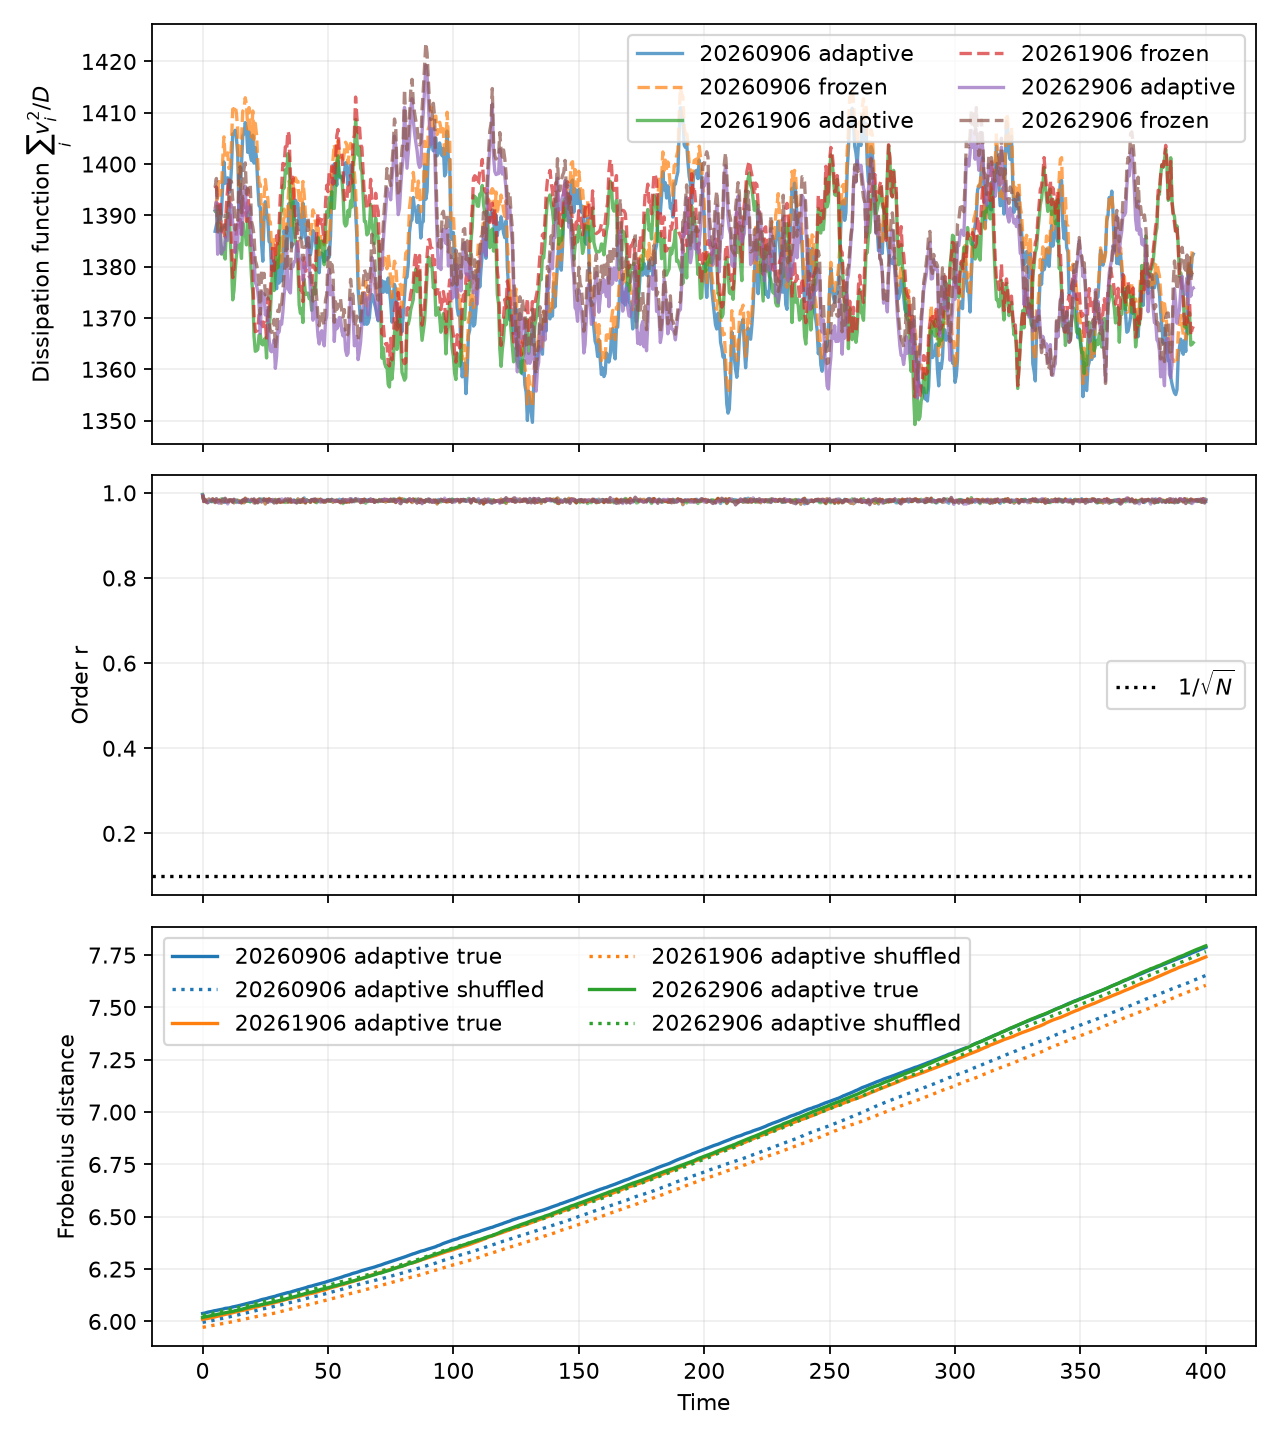
\includegraphics[width=0.85\linewidth,height=0.55\textheight,keepaspectratio]{figures/structural_resonance/joint_dynamics.png}
\caption{Coherence persists while coupling loses alignment with the frequency-cluster template. Gradient updates (solid), random updates (dash-dotted), relabelled gradient updates (dash-dot-dotted), and a frozen kernel (dashed) share one phase-noise stream per seed. Panels show the immediate post-update squared-drift objective, phase order, within-cluster to between-cluster coupling, and template distances. The gradient arm preserves order while its coupling ratio falls; growth in both distances mainly reflects kernel norm. The objective panel samples the instant after updates; complete-interval measurements find no sustained reduction in the bounded study.}
\label{fig:resonance}
\end{figure}

\subsection{What must be specified and measured}

The framework supplies a cover of local states as an argument, with overlap compatibility among its fields. Its proposed physical bridge, E78, connects supercritical coherence to relaxation toward the equilibrium of that cover. For deterministic positive coupling, convergence to a potential minimum is proved under an explicit initial basin condition. Connecting that relaxation to the noisy stationary order parameter requires E78. Compatibility itself is supplied by the cover, so the construction does not explain how initially inconsistent representations become consistent.

A neural test must first identify the domains and objects whose agreement is at issue. Two decoders should estimate a shared content on overlapping domains, with restriction maps specified before inspecting their agreement. Their discrepancy needs a null under decoding noise, and the procedure must distinguish deliberately constructed compatible and incompatible examples. A common prior can make separate decoders agree artificially; region-specific bias can make them disagree artificially. The supplement develops these requirements. An estimator built from phase agreement would miss the property the counterexample separates.

Choosing a cover is also part of choosing a candidate subject. Trivial descriptions can agree while carrying little content, and a suitably chosen partition can conceal disagreement. The scientifically useful choice must therefore be constrained independently by what local activity encodes and which shared quantities can be compared. The uniqueness theorem then answers a precise question about that choice: whether the supplied local descriptions determine one global state. It leaves the empirical selection of domains and descriptions to the model.

\section{Self-representation: a state that models itself}
\label{sec:self}

\subsection{The reflexive construction}

Compatibility yields a global state. Reflexivity adds a relation between that state and an encoding within it. Equip global sections with a complete metric. Under the additional restriction-resonance condition, the encoding of a section $s$ is its restriction to a region $U$, and the map takes the form
\begin{equation}
 F(s)=\operatorname{readout}(s|_U).
 \label{eq:selfmap}
\end{equation}
The same region and readout are used across the model's state space. If $F$ contracts and fixes the section $s_*$ supplied by the cover, Banach's theorem makes $s_*$ its unique fixed point \cite{banach1922}. The formal bridge E89 supplies the contraction law and $F(s_*)=s_*$ for the boundary's encoding--readout composite. Identifying that encoding with restriction is a separate resonance condition; E89 does not supply it. The supercritical order parameter provides an inequality used by the specified contraction bound; constructing the encoding and readout remains a separate obligation.

The point of requiring this particular fixed point is that the self-model refers to the state formed from the local descriptions. A fixed point of an unrelated map would leave that relationship unexplained. The equality expresses accuracy at the level of the modelled state: the encoding reads back the state that contains it. The term \emph{predictive} names this reconstruction map; identifying its operation with a temporal neural prediction requires a dynamical interpretation.

\subsection{Why connect these properties to unity and a minimal self?}
\label{sec:commitment}

We propose two identifications. The section glued from compatible local states is the formal correlate of the unity of a conscious episode. Its accurate self-representation is the formal correlate of a minimal self. These are philosophical commitments, motivated by the relations the construction expresses.

The unity proposal starts from a distinction between having several contents and having several experiences. A globally coherent description can contain many different local contents because compatibility only constrains their shared domains. Gluing makes their contribution to one state explicit. It also demands care about what is encoded. An episode can include uncertainty or conflicting judgments. The relevant question is whether its local descriptions can consistently represent that uncertainty or conflict, rather than whether every represented proposition is true or every judgment agrees. Applying the proposal requires a content model that preserves this distinction.

The self proposal addresses a different feature: the global state has a representation of its own condition within the system that realizes it. A region encoding the surrounding world alone would not meet this requirement. Restriction followed by readout supplies a precise version of internal self-reference, and the fixed-state condition expresses accuracy. In this limited sense the state is what it takes itself to be. Nothing in that description requires a verbal report, an autobiographical narrative or explicit reflection.

Accuracy is a demanding idealization. The construction concerns the variables represented by $s_*$, not an exhaustive internal copy of every microscopic physical fact. A cortical realization would have to specify those variables and justify the fidelity needed for the identification. Approximate self-models, errors and changing states may require a weaker condition than an exact fixed point. Such a condition is a research question rather than a consequence of the theorem.

The relation between the two clauses is itself a commitment. Gluing alone does not require self-representation. The full identification proposes that unified conscious episodes satisfy both clauses, with the self-model about the very state whose unity gluing expresses. The necessity of reflexivity is a philosophical hypothesis, open to dissociation. Unified experience without the proposed self-encoding would count against that requirement, while leaving the compatibility proposal assessable on its own.

\subsection{Which cover and which self-model?}

Both uniqueness results are conditional on their objects. Gluing gives one global extension of specified compatible local data; Banach gives one fixed point of a specified contracting map. These solve ambiguity within a chosen construction. They do not choose between different covers, different encodings or different candidate subjects. Integrated information theory makes exclusion an explicit part of its account \cite{tononi2016}; the present uniqueness results do not settle that selection problem.

The relevant cover and map must be tied to neural organization by evidence independent of the desired conclusion. Local descriptions should predict the contents attributed to their domains; their restrictions should preserve meaning on shared domains; and an encoding region should carry information about the proposed global state that its readout can recover across an independently specified range of states. These are criteria for a biological model, beyond existence of the mathematical objects.

This matters because contraction and a fixed point are easy to obtain in an uninformative construction. A constant readout returning one predetermined state would satisfy those two conditions while explaining little about self-representation. Local encoding and the restriction-resonance condition make the proposed relation explicit, but its psychological significance still depends on a demonstrated relation to the state. An intervention on an encoding should have consequences predicted by that relation. The theory needs this empirical identification as much as it needs calibrated coupling.

\subsection{Dissociations that would bear on the identification}

A test of the full commitment must measure its clauses separately: effective coupling relative to diffusion, overlap compatibility, and the accuracy of the proposed self-encoding, alongside an independent endpoint for experience. A case meeting all three physical and representational conditions with evidence against a unified conscious episode would challenge their sufficiency. Unified experience with demonstrably incompatible local descriptions would challenge the unity identification. Unified experience with compatibility but without the specified self-encoding would challenge the reflexive requirement.

Anesthetic emergence, dreaming and dissociative states are candidate settings because the framework asks whether coordination, unified content and self-representation can separate. Interpreting such evidence requires a declared relation between the experience endpoint and report; absence of report alone cannot define absence of an episode. The compatibility observable in the supplement is a specification, and the corresponding neural self-encoding has yet to be identified. These are the main obstacles to testing the interpretive commitment.

The proposal concerns which state is conscious. It supplies no explanation of why satisfying these relations should be accompanied by experience. Nor do its gluing and fixed-point conditions select an electromagnetic substrate: the cortical field commitment resides in the physical identification and calibration. Their multiple realizability leaves the status of other biological and artificial implementations open.

\section{Thermodynamic constraints and the conditional composition}
\label{sec:chain}

The three requirements can be stated beginning with the phase model. Finite capacity, symmetry breaking and erasure are not needed to derive its stationary threshold. Their role in the broader framework is to constrain a proposed physical implementation: what it can retain, where its degrees of freedom are bounded, and what its updates dissipate. The formal composition asks whether such an implementation can be connected consistently to the coherent, compatible and reflexive state just described. It is one proposed architecture, not a necessary route from thermodynamics to consciousness.

\subsection{Capacity and predictive memory constrain an implementation}

For a finite state space $X$, Shannon entropy satisfies $H(p)\leq\log|X|$, with equality only for the uniform law. A stream with more possible histories than $|X|$ cannot be encoded injectively in that register. Separately, a continuous field on a connected substrate reaching distinct components of a disconnected vacuum manifold must leave that manifold somewhere \cite{kibble1976}. The finite register and the field boundary are independent starting objects. Identifying them as parts of one physical system is an assumption.

A non-surjective update on a finite register is non-injective. Under the specified system--bath model, erasure carries a Landauer heat cost \cite{landauer1961}; connecting logical many-to-one processing to physical heat requires implementation assumptions \cite{norton2005,shenker2000}. For a state $X_t$ driven by an environmental signal $S_t$, the predictive dissipation bound is
\begin{equation}
 W_{\mathrm{diss}}\geq k_BT\left[I(X_t;S_t)-I(X_t;S_{t+1})\right].
 \label{eq:predictive}
\end{equation}
Under the no-back-action Markov structure $X_t\to S_t\to S_{t+1}$, the bracket is nonnegative \cite{still2012}. The bound limits nonpredictive memory at a given dissipation budget. Deriving it from the register's Landauer bound requires the nonpredictive information to be bounded by the entropy erased, with the same thermal scale and heat budget.

This constrains memory without specifying its content or learning rule. Zero retained information can satisfy the bound, so reducing its right-hand side does not require better representation. A bound $D_{KL}\leq\Delta t\,\sigma$ forces convergence of $D_{KL}$ to zero only when its right-hand side tends to zero. Counting capacity, erased entropy and predictive mutual information have different roles \cite{rosas2026}. The plasticity control makes the consequence concrete: an objective must be related to the structure a system is expected to learn.

\subsection{What the composition establishes}

Table~\ref{tab:summary} lists the eight implications accepted by the theorem \texttt{chain}. Its node predicates concern finite capacity, a symmetry-breaking boundary, erasure heat, a predictive dissipation bound, a continuum coupling limit, a physical field realization, coherent order, a glued section and a reflexive fixed point. The ordering specifies the theorem's arguments. In particular, the implication from finite capacity to a boundary is supplied independently; the ordering does not turn it into a deduction.

\begin{table}[htbp]
\centering
\singlespacing
\small
\begin{tabular}{>{\raggedright\arraybackslash}p{0.14\linewidth}>{\raggedright\arraybackslash}p{0.20\linewidth}>{\raggedright\arraybackslash}p{0.56\linewidth}}
\hline
Connection & Status & Required assumption \\
\hline
E12 & Independent physical premise & A finite-capacity system realizes a field that leaves its vacuum manifold. Capacity and the boundary are independent roots. \\
E23 & Bridge assumption & The boundary is associated with a finite register whose update leaves states unreachable. \\
E34 & Bridge assumption & Erasure supplies a predictive structure with the same thermal scale and heat budget, and nonzero wasted memory. \\
E45 & Modelling assumption & The predictive dissipation bound places coupling energies in a convergent coarse-graining regime. \\
E56 & Physical commitment & A specified physical field realizes the limiting coupling and satisfies the kernel conditions. \\
E67 & Physical commitment & That field operates above the synchronization threshold. \\
E78 & Bridge assumption & Coherence drives a supplied cover to its relaxed equilibrium at coupling at least the named mean-field value. \\
E89 & Modelling assumption & A contracting map mediated by local self-encoding fixes the section glued on that same cover. \\
\hline
\end{tabular}
\caption{Connecting hypotheses of the formal composition. The cover's compatibility is supplied as a structure field. Identifying the boundary's encoding with restriction requires a separate resonance condition. The mathematical objects and node-level results are mapped in Supplemental Material, Table~S1.}
\label{tab:summary}
\end{table}

Two structures also enter the theorem: a thermodynamic cover, including overlap compatibility, and a reflexive boundary specifying the local encoding and readout. Given these structures and the connecting hypotheses, \texttt{chain} concludes \texttt{UnifiedSelf}: the particular section glued on that cover is the unique fixed point of self-prediction. The theorem does not require the separate restriction-resonance predicate; that condition is needed to interpret its encoding as the restriction in Eq.~\eqref{eq:selfmap}. The conclusion binds the endpoint to the supplied objects; its interpretation as a conscious state is the commitment of Section~\ref{sec:commitment}.

The formal development includes a joint witness assembled from a double well, a register, a uniform-grid mesh and a three-site cortex. It establishes that the hypotheses can hold together, while the components remain distinct toy systems. Counterexamples such as phase agreement without compatible profiles expose the work individual assumptions do. The development declares no additional Lean axioms beyond the foundational axioms used by its libraries; physical content is carried by hypotheses and model fields. This makes the conditional construction checkable without treating a biological premise as a proved fact.

\section{Discussion}

This construction separates three proposed requirements for conscious unity: collective timing, compatible local descriptions and an accurate representation of the resulting global state. Each answers a different question. Coupling can sustain coherence; gluing gives one state from specified compatible descriptions; and reflexivity relates that state to an encoding within itself.

The physical proposal is a geometry-mediated increase in effective coupling during awakening. Its most useful experimental consequence is a hierarchy of measurements. Concentration and coherence test a phase-density description. Resolved increments add rate information. A measured drive or selective perturbation is needed to distinguish interaction mechanisms. Finite ramps determine how the transition appears, so a fitted onset exponent cannot substitute for those measurements. Calibration and identifiability govern what a recovery experiment can conclude.

The representational proposal begins where a synchronization account runs out of explanatory content. Equal phases permit disagreement on overlaps, and the specified plasticity rule can sustain coherence while moving away from environmental alignment. The framework therefore assigns compatibility its own mathematical condition and measurement task. A biological account must explain which local descriptions carry relevant content and how their agreement is maintained. Thermodynamic bounds constrain this account without supplying the missing content model.

The reflexive proposal adds an internal representation of the same global state. Its appeal is the explicit relationship between unity and self-reference; its cost is the need to identify a cover and encoding independently, justify the accuracy idealization and test whether unified experience requires that relation. These are substantive commitments left open by uniqueness relative to fixed mathematical objects.

Compared with integrated information, global-workspace and predictive-processing accounts \cite{tononi2016,baars1997,dehaene2014,friston2010}, the framework places a candidate physical interaction beside a compatibility condition and a local self-encoding. Its contribution is a conditional connection between them, with concrete examples of where simpler inferences fail. The next decisive evidence would couple a calibrated recovery experiment to independently validated measures of content compatibility and self-representation. Together those measurements would ask whether the cortical state that becomes coordinated is also the state that fits together and represents itself.

\section*{Data and code availability}

The Lean development, simulation scripts, tests and saved numerical summaries are maintained in the \href{https://github.com/bobaseb/coupling_gated_cortical_coherence}{manuscript source repository}. Publication simulation values are regenerated from saved summaries without rerunning production sweeps. The exploratory EEG analysis uses OpenNeuro dataset ds005620 \cite{bajwa2025}; preprocessing and selection are described in Supplemental Material. The source repository contains the reproducible analysis and does not redistribute the raw recordings.

\section*{Funding and competing interests}

This research received no external funding. The author declares no competing interests.

\section*{Use of AI tools}

AI assistance to this work was substantial and is not separable by task. Several coding assistants and chat interfaces were used in an interleaved way throughout: Google's Antigravity CLI (Gemini 3.1, Claude 4.6 Opus, Claude 4.6 Sonnet), OpenAI's Codex CLI (Astra, Terra, Luna, Sol), Claude Code (Claude Opus 5), Gemini Pro through its web interface, and Fable (Claude Opus 4) through OpenRouter, accessed with the Hermes CLI. Between them they contributed to the Lean development, the simulation and analysis code, and the drafting and revision of both documents. Because the tools were used in combination and in alternation, no section, proof, figure or result is attributable to any one of them, and none is claimed to be. The author is responsible for all content, including everything a tool produced. Machine checking establishes the stated Lean results under their hypotheses; it does not validate biological interpretations or replace scientific review of generated code and prose.


\begin{thebibliography}{99}

\bibitem[Pinotsis \& Miller(2022)]{pinotsis2022}
 Pinotsis, D. A., \& Miller, E. K. (2022). Beyond dimension reduction: Stable electric fields emerge from and allow representational drift. \textit{NeuroImage}, 253, 119058.

\bibitem[Tononi et al.(2016)]{tononi2016}
 Tononi, G., Boly, M., Massimini, M., \& Koch, C. (2016). Integrated information theory: from consciousness to its physical substrate. \textit{Nature Reviews Neuroscience}, 17(7), 450-461.

\bibitem[Singer \& Gray(1995)]{singer1995}
 Singer, W., \& Gray, C. M. (1995). Visual feature integration and the temporal correlation hypothesis. \textit{Annual Review of Neuroscience}, 18, 555-586.

\bibitem[Fries(2015)]{fries2015}
 Fries, P. (2015). Rhythms for cognition: communication through coherence. \textit{Neuron}, 88(1), 220-235.

\bibitem[Shadlen \& Movshon(1999)]{shadlen1999}
 Shadlen, M. N., \& Movshon, J. A. (1999). Synchrony unbound: a critical evaluation of the temporal binding hypothesis. \textit{Neuron}, 24(1), 67-77.

\bibitem[Tsuchiya et al.(2015)]{tsuchiya2015}
 Tsuchiya, N., Wilke, M., Fr\"{a}ssle, S., \& Lamme, V. A. F. (2015). No-report paradigms: extracting the true neural correlates of consciousness. \textit{Trends in Cognitive Sciences}, 19(12), 757-770.

\bibitem[Metzinger(2003)]{metzinger2003}
 Metzinger, T. (2003). \textit{Being No One: The Self-Model Theory of Subjectivity}. Cambridge, MA: MIT Press.

\bibitem[Seth(2013)]{seth2013}
 Seth, A. K. (2013). Interoceptive inference, emotion, and the embodied self. \textit{Trends in Cognitive Sciences}, 17(11), 565-573.

\bibitem[Butlin et al.(2023)]{butlin2023}
 Butlin, P., Long, R., Elmoznino, E., Bengio, Y., Birch, J., et al. (2023). Consciousness in artificial intelligence: insights from the science of consciousness. \textit{arXiv preprint} arXiv:2308.08708.

\bibitem[Bobadilla-Suarez et al.(2020)]{bobadillasuarez2020}
 Bobadilla-Suarez, S., Ahlheim, C., Mehrotra, A., Panos, A., \& Love, B. C. (2020). Measures of neural similarity. \textit{Computational Brain \& Behavior}, 3, 369-383.

\bibitem[DiCarlo \& Cox(2007)]{dicarlo2007}
 DiCarlo, J. J., \& Cox, D. D. (2007). Untangling invariant object recognition. \textit{Trends in Cognitive Sciences}, 11(8), 333-341.

\bibitem[Kriegeskorte \& Diedrichsen(2019)]{kriegeskorte2019}
 Kriegeskorte, N., \& Diedrichsen, J. (2019). Peeling the onion of brain representations. \textit{Annual Review of Neuroscience}, 42, 407-432.

\bibitem[Gallagher(2000)]{gallagher2000}
 Gallagher, S. (2000). Philosophical conceptions of the self: implications for cognitive science. \textit{Trends in Cognitive Sciences}, 4(1), 14-21.

\bibitem[Baars(1997)]{baars1997}
 Baars, B. J. (1997). In the Theater of Consciousness: The Workspace of the Mind. \textit{Oxford University Press}.

\bibitem[Dehaene et al.(2014)]{dehaene2014}
 Dehaene, S., Charles, L., King, J. R., \& Marti, S. (2014). Toward a computational theory of conscious processing. \textit{Current Opinion in Neurobiology}, 25, 76-84.

\bibitem[Friston(2010)]{friston2010}
 Friston, K. (2010). The free-energy principle: a unified brain theory?. \textit{Nature Reviews Neuroscience}, 11(2), 127-138.

\bibitem[Milinkovic \& Aru(2026)]{milinkovic2026}
 Milinkovic, B., \& Aru, J. (2026). On biological and artificial consciousness: A case for biological computationalism. \textit{Neuroscience \& Biobehavioral Reviews}, 181, 106524. \href{https://doi.org/10.1016/j.neubiorev.2025.106524}{doi:10.1016/j.neubiorev.2025.106524}.

\bibitem[Aru et al.(2023)]{aru2023}
 Aru, J., Larkum, M. E., \& Shine, J. M. (2023). The feasibility of artificial consciousness through the lens of neuroscience. \textit{Trends in Neurosciences}, 46(12), 1008--1017. \href{https://doi.org/10.1016/j.tins.2023.09.009}{doi:10.1016/j.tins.2023.09.009}.

\bibitem[Seth(2026a)]{seth2026}
 Seth, A. K. (2026). Conscious artificial intelligence and biological naturalism. \textit{Behavioral and Brain Sciences}, 49, e315. \href{https://doi.org/10.1017/S0140525X25000032}{doi:10.1017/S0140525X25000032}.

\bibitem[Seth(2026b)]{seth2026response}
 Seth, A. K. (2026). The stuff matters: Consciousness, computation, and biology. \textit{Behavioral and Brain Sciences}, 49, e366. \href{https://doi.org/10.1017/S0140525X26106906}{doi:10.1017/S0140525X26106906}.

\bibitem[Gurnee et al.(2026)]{gurnee2026}
 Gurnee, W., et al. (2026). Verbalizable Representations Form a Global Workspace in Language Models. \textit{Transformer Circuits Thread}. \href{https://arxiv.org/abs/2607.15495}{arXiv:2607.15495}.

\bibitem[Aguilera et al.(2022)]{aguilera2022}
 Aguilera, M., Millidge, B., Tschantz, A., \& Buckley, C. L. (2022). How particular is the physics of the free energy principle?. \textit{Physics of Life Reviews}, 40, 24-50.

\bibitem[Biehl et al.(2021)]{biehl2021}
 Biehl, M., Pollock, F. A., \& Kanai, R. (2021). A technical critique of some parts of the free energy principle. \textit{Entropy}, 23(3), 293.

\bibitem[Bruineberg et al.(2022)]{bruineberg2022}
 Bruineberg, J., Dolega, K., Dewhurst, J., \& Baltieri, M. (2022). The Emperor's New Markov Blankets. \textit{Behavioral and Brain Sciences}, 45, e183.

\bibitem[Pinotsis \& Miller(2023a)]{pinotsis2023ephaptic}
 Pinotsis, D. A., \& Miller, E. K. (2023). In vivo ephaptic coupling allows memory network formation. \textit{Cerebral Cortex}, 33(17), 9877-9895.

\bibitem[Pinotsis \& Miller(2023b)]{pinotsis2023cytoelectric}
 Pinotsis, D. A., Fridman, G., \& Miller, E. K. (2023). Cytoelectric coupling: Electric fields sculpt neural activity and "tune" the brain's infrastructure. \textit{Progress in Neurobiology}, 226, 102465.

\bibitem[McFadden(2002)]{mcfadden2002}
 McFadden, J. (2002). The conscious electromagnetic information (cemi) field theory: the hard problem made easy?. \textit{Journal of Consciousness Studies}, 9(8), 45-60.

\bibitem[Pockett(2012)]{pockett2012}
 Pockett, S. (2012). The electromagnetic field theory of consciousness: a testable hypothesis about the characteristics of conscious as opposed to non-conscious fields. \textit{Journal of Consciousness Studies}, 19(11-12), 191-223.

\bibitem[McFadden(2020)]{mcfadden2020}
 McFadden, J. (2020). Integrating information in the brain's EM field: the cemi field theory of consciousness. \textit{Neuroscience of Consciousness}, 2020(1), niaa016.

\bibitem[Fr\"{o}hlich \& McCormick(2010)]{frohlich2010}
 Fr\"{o}hlich, F., \& McCormick, D. A. (2010). Endogenous electric fields may guide neocortical network activity. \textit{Neuron}, 67(1), 129-143.

\bibitem[Anastassiou \& Koch(2015)]{anastassiou2015}
 Anastassiou, C. A., \& Koch, C. (2015). Ephaptic coupling to endogenous electric field activity: why bother?. \textit{Current Opinion in Neurobiology}, 31, 95-103.

\bibitem[Pockett(2002)]{pockett2002}
 Pockett, S. (2002). Difficulties with the electromagnetic field theory of consciousness. \textit{Journal of Consciousness Studies}, 9(4), 51-56.

\bibitem[V\"or\"oslakos et al.(2018)]{voroslakos2018}
 V\"or\"oslakos, M., et al. (2018). Direct effects of transcranial electric stimulation on brain circuits in rats and humans. \textit{Nature Communications}, 9, 483.

\bibitem[Verkhratsky \& Nedergaard(2018)]{verkhratsky2018}
 Verkhratsky, A., \& Nedergaard, M. (2018). Physiology of Astroglia. \textit{Physiological Reviews}, 98(1), 239-389.

\bibitem[Mountcastle(1997)]{mountcastle1997}
 Mountcastle, V. B. (1997). The columnar organization of the neocortex. \textit{Brain}, 120(4), 701-722. \href{https://doi.org/10.1093/brain/120.4.701}{doi:10.1093/brain/120.4.701}.

\bibitem[Horton \& Adams(2005)]{horton2005}
 Horton, J. C., \& Adams, D. L. (2005). The cortical column: a structure without a function. \textit{Philosophical Transactions of the Royal Society B}, 360(1456), 837-862. \href{https://doi.org/10.1098/rstb.2005.1623}{doi:10.1098/rstb.2005.1623}.

\bibitem[Rakic(2008)]{rakic2008}
 Rakic, P. (2008). Confusing cortical columns. \textit{Proceedings of the National Academy of Sciences}, 105(34), 12099-12100. \href{https://doi.org/10.1073/pnas.0807271105}{doi:10.1073/pnas.0807271105}.

\bibitem[Bastos et al.(2021)]{bastos2021}
 Bastos, A. M., Donoghue, J. A., Brincat, S. L., Mahnke, M., Yanar, J., Correa, J., ... \& Miller, E. K. (2021). Neural effects of propofol-induced unconsciousness and its reversal using thalamic stimulation. \textit{eLife}, 10, e60824.

\bibitem[Bajwa et al.(2025)]{bajwa2025}
   Bajwa, I. J., Nilsen, A. S., Skukies, R., Aamodt, A., Ernst, G., Storm, J. F., \& Juel, B. E. (2025). A repeated awakening study exploring the capacity of complexity measures to capture dreaming during propofol sedation. \textit{Scientific Reports}, 15, 32746. \href{https://doi.org/10.1038/s41598-025-12695-z}{doi:10.1038/s41598-025-12695-z}.

\bibitem[Xie et al.(2013)]{xie2013}
 Xie, L., Kang, H., Xu, Q., Chen, M. J., Liao, Y., Thiyagarajan, M., ... \& Nedergaard, M. (2013). Sleep drives metabolite clearance from the adult brain. \textit{Science}, 342(6156), 373-377.

\bibitem[Sykov\'{a} \& Nicholson(2008)]{sykova2008}
 Sykov\'{a}, E., \& Nicholson, C. (2008). Diffusion in brain extracellular space. \textit{Physiological Reviews}, 88(4), 1277-1340.

\bibitem[Barbour(2017)]{barbour2017}
 Barbour, B. (2017). Analysis of claims that the brain extracellular impedance is high and non-resistive. \textit{Biophysical Journal}, 113(7), 1636-1638.

\bibitem[Logothetis et al.(2007)]{logothetis2007}
 Logothetis, N. K., Kayser, C., \& Oeltermann, A. (2007). In vivo measurement of cortical impedance spectrum in monkeys: implications for signal propagation. \textit{Neuron}, 55(5), 809--823. \href{https://doi.org/10.1016/j.neuron.2007.07.027}{doi:10.1016/j.neuron.2007.07.027}.

\bibitem[Gabriel et al.(1996)]{gabriel1996}
 Gabriel, S., Lau, R. W., \& Gabriel, C. (1996). The dielectric properties of biological tissues: II. Measurements in the frequency range 10 Hz to 20 GHz. \textit{Physics in Medicine and Biology}, 41(11), 2251--2269. \href{https://doi.org/10.1088/0031-9155/41/11/002}{doi:10.1088/0031-9155/41/11/002}.

\bibitem[Norton(2005)]{norton2005}
 Norton, J. D. (2005). Eaters of the lotus: Landauer's principle and the return of Maxwell's demon. \textit{Studies in History and Philosophy of Science Part B: Studies in History and Philosophy of Modern Physics}, 36(2), 375-411.

\bibitem[Landauer(1961)]{landauer1961}
 Landauer, R. (1961). Irreversibility and heat generation in the computing process. \textit{IBM Journal of Research and Development}, 5(3), 183-191.

\bibitem[Kibble(1976)]{kibble1976}
 Kibble, T. W. B. (1976). Topology of cosmic domains and strings. \textit{Journal of Physics A: Mathematical and General}, 9(8), 1387-1398.

\bibitem[Sakaguchi(1988)]{sakaguchi1988}
 Sakaguchi, H. (1988). Cooperative phenomena in coupled oscillator systems under external fields. \textit{Progress of Theoretical Physics}, 79(1), 39-46.

\bibitem[Strogatz \& Mirollo(1991)]{strogatz1991}
 Strogatz, S. H., \& Mirollo, R. E. (1991). Stability of incoherence in a population of coupled oscillators. \textit{Journal of Statistical Physics}, 63, 613--635.

\bibitem[Acebr\'{o}n et al.(2005)]{acebron2005}
 Acebr\'{o}n, J. A., Bonilla, L. L., P\'{e}rez Vicente, C. J., Ritort, F., \& Spigler, R. (2005). The Kuramoto model: A simple paradigm for synchronization phenomena. \textit{Reviews of Modern Physics}, 77, 137--185. \href{https://doi.org/10.1103/RevModPhys.77.137}{doi:10.1103/RevModPhys.77.137}.

\bibitem[Ott \& Antonsen(2008)]{ott2008}
 Ott, E., \& Antonsen, T. M. (2008). Low dimensional behavior of large systems of globally coupled oscillators. \textit{Chaos}, 18, 037113. \href{https://doi.org/10.1063/1.2930766}{doi:10.1063/1.2930766}.

\bibitem[D\"orfler \& Bullo(2014)]{dorfler2014}
 D\"orfler, F., \& Bullo, F. (2014). Synchronization in complex networks of phase oscillators: A survey. \textit{Automatica}, 50, 1539--1564. \href{https://doi.org/10.1016/j.automatica.2014.04.012}{doi:10.1016/j.automatica.2014.04.012}.

\bibitem[Breakspear(2017)]{breakspear2017}
 Breakspear, M. (2017). Dynamic models of large-scale brain activity. \textit{Nature Neuroscience}, 20, 340--352. \href{https://doi.org/10.1038/nn.4497}{doi:10.1038/nn.4497}.

\bibitem[Still et al.(2012)]{still2012}
 Still, S., Sivak, D. A., Bell, A. J., \& Crooks, G. E. (2012). Thermodynamics of prediction. \textit{Physical Review Letters}, 109(12), 120604.

\bibitem[Kawai et al.(2007)]{kawai2007}
 Kawai, R., Parrondo, J. M. R., \& Van den Broeck, C. (2007). Dissipation: The phase-space perspective. \textit{Physical Review Letters}, 98(8), 080602.

\bibitem[Horowitz and Esposito(2014)]{horowitz2014}
 Horowitz, J. M., \& Esposito, M. (2014). Thermodynamics with continuous information flow. \textit{Physical Review X}, 4, 031015. \href{https://doi.org/10.1103/PhysRevX.4.031015}{doi:\allowbreak10.1103/\allowbreak PhysRevX.4.\allowbreak031015}.

\bibitem[Ito and Sagawa(2013)]{ito2013}
 Ito, S., \& Sagawa, T. (2013). Information thermodynamics on causal networks. \textit{Physical Review Letters}, 111, 180603. \href{https://doi.org/10.1103/PhysRevLett.111.180603}{doi:\allowbreak10.1103/\allowbreak PhysRevLett.111.\allowbreak180603}.

\bibitem[Corberi et al.(2026)]{corberi2026}
 Corberi, F., dello Russo, S., Messuti, G., Scarpetta, S., \& Smaldone, L. (2026). Thermodynamic learning. \textit{arXiv preprint}. \href{https://arxiv.org/abs/2609.04732}{arXiv:2609.04732}.

\bibitem[Banach(1922)]{banach1922}
 Banach, S. (1922). Sur les op\'{e}rations dans les ensembles abstraits et leur application aux \'{e}quations int\'{e}grales. \textit{Fundamenta Mathematicae}, 3(1), 133-181.

\bibitem[Shenker(2000)]{shenker2000}
  Shenker, O. R. (2000). Logic and entropy. \textit{PhilSci-Archive preprint}. \href{https://philsci-archive.pitt.edu/115/}{philsci-archive.pitt.edu/115}.

\bibitem[Rosas et al.(2026)]{rosas2026}
  Rosas, F. E., Mediano, P. A. M., Luppi, A. I., Boyd, A. B., Berta, M., Jensen, H. J., Gastpar, M., \& Carroll, S. M. (2026). Four faces of information in natural systems. \textit{Nature Reviews Physics}. \href{https://doi.org/10.1038/s42254-026-00971-4}{doi:10.1038/s42254-026-00971-4}.

\bibitem[Sznitman(1991)]{sznitman1991}
  Sznitman, A.-S. (1991). Topics in propagation of chaos. In \textit{\'Ecole d'\'Et\'e de Probabilit\'es de Saint-Flour XIX---1989}, Lecture Notes in Mathematics, vol.~1464, pp.~165--251. Springer. \href{https://doi.org/10.1007/BFb0085169}{doi:10.1007/BFb0085169}.

\bibitem[Dai Pra \& den Hollander(1996)]{daipra1996}
 Dai Pra, P., \& den Hollander, F. (1996). McKean--Vlasov limit for interacting random processes in random media. \textit{Journal of Statistical Physics}, 84, 735--772. \href{https://doi.org/10.1007/BF02179656}{doi:10.1007/BF02179656}.

\bibitem[Bertini et al.(2010)]{bertini2010}
 Bertini, L., Giacomin, G., \& Pakdaman, K. (2010). Dynamical aspects of mean field plane rotators and the Kuramoto model. \textit{Journal of Statistical Physics}, 138, 270--290. \href{https://doi.org/10.1007/s10955-009-9908-9}{doi:10.1007/s10955-009-9908-9}.

\bibitem[Berglund \& Gentz(2002)]{berglund2002}
  Berglund, N., \& Gentz, B. (2002). Pathwise description of dynamic pitchfork bifurcations with additive noise. \textit{Probability Theory and Related Fields}, 122, 341--388. \href{https://doi.org/10.1007/s004400100174}{doi:10.1007/s004400100174}.

\bibitem[Abramsky \& Brandenburger(2011)]{abramsky2011}
  Abramsky, S., \& Brandenburger, A. (2011). The sheaf-theoretic structure of non-locality and contextuality. \textit{New Journal of Physics}, 13, 113036. \href{https://doi.org/10.1088/1367-2630/13/11/113036}{doi:10.1088/1367-2630/13/11/113036}.

\bibitem[Townsend et al.(2015)]{townsend2015}
 Townsend, R. G., Solomon, S. S., Chen, S. C., Pietersen, A. N. J., Martin, P. R., Solomon, S. G., \& Gong, P. (2015). Emergence of complex wave patterns in primate cerebral cortex. \textit{The Journal of Neuroscience}, 35(11), 4657-4662. \href{https://doi.org/10.1523/JNEUROSCI.4509-14.2015}{doi:10.1523/JNEUROSCI.4509-14.2015}.

\bibitem[Xu et al.(2023)]{xu2023}
 Xu, Y., Long, X., Feng, J., \& Gong, P. (2023). Interacting spiral wave patterns underlie complex brain dynamics and are related to cognitive processing. \textit{Nature Human Behaviour}, 7(7), 1196-1215. \href{https://doi.org/10.1038/s41562-023-01626-5}{doi:10.1038/s41562-023-01626-5}.

\bibitem[Nicoletti et al.(2026)]{nicoletti2026}
 Nicoletti, G., Di Terlizzi, I., \& Busiello, D. M. (2026). Balancing information and dissipation with partially observed fluctuating signals. \textit{Physical Review Letters}, 137(12), 127101. \href{https://doi.org/10.1103/8gx2-rbns}{doi:10.1103/8gx2-rbns}.

\bibitem[Kiyooka et al.(2026)]{kiyooka2026}
 Kiyooka, D., Oomoto, I., Kitazono, J., Saito, Y., Kobayashi, M., Matsubara, C., Kobayashi, K., Murayama, M., \& Oizumi, M. (2026). Single-cell resolution functional networks during unconsciousness are segregated into spatially intermixed modules. \textit{Cell Reports}, 45(2), 116902. \href{https://doi.org/10.1016/j.celrep.2025.116902}{doi:10.1016/j.celrep.2025.116902}.

\bibitem[Oomoto et al.(2026)]{oomoto2026}
 Oomoto, I., Kiyooka, D., Oizumi, M., \& Murayama, M. (2026). Multi-area single-cell calcium imaging dataset of the mouse cortex across wakefulness, sleep, and anesthesia. \textit{Scientific Data}. \href{https://doi.org/10.1038/s41597-026-08202-2}{doi:10.1038/s41597-026-08202-2}.

\bibitem[Attwell \& Laughlin(2001)]{attwell2001}
 Attwell, D., \& Laughlin, S. B. (2001). An energy budget for signaling in the grey matter of the brain. \textit{Journal of Cerebral Blood Flow \& Metabolism}, 21(10), 1133-1145. \href{https://doi.org/10.1097/00004647-200110000-00001}{doi:10.1097/00004647-200110000-00001}.

\bibitem[Harris et al.(2012)]{harris2012}
 Harris, J. J., Jolivet, R., \& Attwell, D. (2012). Synaptic energy use and supply. \textit{Neuron}, 75(5), 762-777. \href{https://doi.org/10.1016/j.neuron.2012.08.019}{doi:10.1016/j.neuron.2012.08.019}.

\bibitem[Nicholls \& Ferguson(2013)]{nicholls2013}
 Nicholls, D. G., \& Ferguson, S. J. (2013). \textit{Bioenergetics 4}. Academic Press.


\bibitem[Baer et al.(1989)]{baer1989}
 Baer, S. M., Erneux, T., \& Rinzel, J. (1989). The slow passage through a Hopf bifurcation: delay, memory effects, and resonance. \textit{SIAM Journal on Applied Mathematics}, 49(1), 55--71. \href{https://doi.org/10.1137/0149003}{doi:10.1137/0149003}.

\bibitem[Friedman et al.(2010)]{friedman2010}
 Friedman, E. B., Sun, Y., Moore, J. T., Hung, H.-T., Meng, Q. C., Perera, P., Joiner, W. J., Thomas, S. A., Eckenhoff, R. G., Sehgal, A., \& Kelz, M. B. (2010). A conserved behavioral state barrier impedes transitions between anesthetic-induced unconsciousness and wakefulness: evidence for neural inertia. \textit{PLoS ONE}, 5(7), e11903. \href{https://doi.org/10.1371/journal.pone.0011903}{doi:10.1371/journal.pone.0011903}.

\bibitem[Hudson et al.(2014)]{hudson2014}
 Hudson, A. E., Calderon, D. P., Pfaff, D. W., \& Proekt, A. (2014). Recovery of consciousness is mediated by a network of discrete metastable activity states. \textit{Proceedings of the National Academy of Sciences}, 111(25), 9283--9288. \href{https://doi.org/10.1073/pnas.1408296111}{doi:10.1073/pnas.1408296111}.

\bibitem[Proekt \& Hudson(2018)]{proekt2018}
 Proekt, A., \& Hudson, A. E. (2018). A stochastic basis for neural inertia in emergence from general anaesthesia. \textit{British Journal of Anaesthesia}, 121(1), 86--94. \href{https://doi.org/10.1016/j.bja.2018.02.035}{doi:10.1016/j.bja.2018.02.035}.
\end{thebibliography}


\end{document}
